\documentclass[conference]{IEEEtran}
\usepackage{amsmath,amssymb}
\usepackage{graphicx}
\usepackage{booktabs}
\usepackage{multirow}

\begin{document}

\title{K-SVD Dictionary Learning: Reproduction and Extension
       to Image Denoising\\
{\large ECE 417 / ECE 613 Final Project --- Winter 2026}}
\author{\IEEEauthorblockN{[Your Name(s)]}
\IEEEauthorblockA{Department of Electrical and Computer Engineering\\
University of Waterloo, Waterloo, ON, Canada}}
\maketitle

\begin{abstract}
We reproduce the K-SVD algorithm of Aharon, Elad, and
Bruckstein~\cite{aharon2006ksvd}, which learns an over-complete
dictionary from training signals using an alternating sparse-coding
and rank-1 SVD update strategy.
Following the paper's synthetic dictionary-recovery experiment,
our implementation recovers $45.5\pm2.2$ out of 50 atoms in the
noiseless case (vs.\ $44.1\pm1.9$ for the MOD baseline), and
performs comparably or better than MOD across all tested noise
levels, reproducing the paper's key qualitative finding.
As a novel extension, we apply the learned-dictionary framework
to image denoising---a problem not addressed in the original
paper---and compare against Non-Local Means (NLM).
We further propose a combined NLM+K-SVD pipeline where NLM
pre-filtering provides cleaner training data for the dictionary,
which improves over standalone K-SVD on smooth images and
consistently outperforms NLM across both test images.
\end{abstract}

\begin{IEEEkeywords}
Dictionary learning, K-SVD, sparse representation, orthogonal
matching pursuit, image denoising, overcomplete dictionaries.
\end{IEEEkeywords}

% ==============================================================
\section{Introduction and Background}
% ==============================================================

Sparse representation has become a foundational tool in signal
processing and image analysis.
The central idea is that natural signals can be well approximated
as sparse linear combinations of a small set of \emph{atoms}
drawn from an over-complete \emph{dictionary}~\cite{mallat1993matching}.
Early work used fixed, analytically designed dictionaries such as
wavelets and DCT bases, which are efficient but not adapted to
the signal class of interest.

\textbf{Dictionary learning} addresses this limitation by jointly
optimising the dictionary and the sparse coefficients from a set
of training signals.
Olshausen and Field~\cite{olshausen1996sparse} showed that
learning a dictionary from image patches recovers Gabor-like
features resembling receptive fields in primary visual cortex.
The Method of Optimal Directions (MOD)~\cite{engan1999mod}
formulated dictionary learning as an alternating minimisation,
updating the dictionary globally via the pseudoinverse.

Aharon, Elad, and Bruckstein~\cite{aharon2006ksvd} introduced
K-SVD, a more efficient alternating algorithm that updates each
dictionary atom individually using a rank-1 singular value
decomposition (SVD) of the corresponding residual matrix.
K-SVD generalises K-means clustering and has been applied to
image compression, inpainting, and---in follow-up
work~\cite{elad2006denoising}---image denoising.
For denoising, Non-Local Means (NLM)~\cite{buades2005nlm}
represents a classical baseline that exploits non-local
self-similarity rather than a learned dictionary.

\textbf{This project} reproduces the synthetic dictionary-recovery
experiment of~\cite{aharon2006ksvd} (Section~V-A), comparing
K-SVD with MOD as the paper's primary baseline.
We then extend K-SVD to image denoising---a problem the original
paper does not address---compare it against NLM, and propose a
combined NLM+K-SVD pipeline that improves over both.

% ==============================================================
\section{Reproducible Component: K-SVD Algorithm}
% ==============================================================

\subsection{Algorithm}

The K-SVD algorithm~\cite{aharon2006ksvd} solves:
\begin{equation}
    \min_{\mathbf{D},\,\mathbf{X}}
    \|\mathbf{Y} - \mathbf{D}\mathbf{X}\|_F^2
    \quad\text{s.t.}\quad
    \forall i:\;\|\mathbf{x}_i\|_0 \leq L,
    \label{eq:ksvd_obj}
\end{equation}
where $\mathbf{Y}\!\in\!\mathbb{R}^{n\times N}$ is the training
matrix, $\mathbf{D}\!\in\!\mathbb{R}^{n\times K}$ the dictionary,
and $\mathbf{X}\!\in\!\mathbb{R}^{K\times N}$ the sparse codes.
K-SVD alternates between two steps.

\textbf{Step 1 -- Sparse Coding.}
With $\mathbf{D}$ fixed, each $\mathbf{y}_i$ is encoded by OMP~\cite{pati1993omp} with sparsity $L$.

\textbf{Step 2 -- Dictionary Update.}
For each atom $\mathbf{d}_k$, let $\Omega_k=\{i:x_{k,i}\neq 0\}$
and form the partial residual
\begin{equation}
    \mathbf{E}_k =
    \mathbf{Y}_{\Omega_k}
    - \textstyle\sum_{j\neq k}\mathbf{d}_j\mathbf{x}_j^\top\big|_{\Omega_k}.
\end{equation}
The SVD $\mathbf{E}_k=\mathbf{U\Sigma V}^\top$ gives the updated
atom $\mathbf{d}_k\leftarrow\mathbf{u}_1$ and updated coefficients
$\mathbf{x}_k|_{\Omega_k}\leftarrow\sigma_1\mathbf{v}_1$.
This rank-1 step guarantees non-increasing reconstruction error.

MOD~\cite{engan1999mod} uses the same OMP step but replaces the
column-by-column update with a single global pseudoinverse step:
$\mathbf{D}\leftarrow\mathbf{Y}\mathbf{X}^\dagger$.

\subsection{Experimental Setup}

We follow Section~V-A of~\cite{aharon2006ksvd} exactly:
a true dictionary $\mathbf{D}_0\!\in\!\mathbb{R}^{20\times50}$
with unit-norm Gaussian columns; $N=1500$ signals each built from
$L=3$ randomly chosen atoms with Gaussian weights; additive
Gaussian noise at SNR$\,\in\{\infty,30,20,10\}$\,dB; 80
iterations; 20 Monte Carlo trials.
An atom $\hat{\mathbf{d}}$ is \emph{recovered} when
$\max_k|\hat{\mathbf{d}}^\top\mathbf{d}_{0,k}|\geq 1-\varepsilon$
($\varepsilon=0.01$).

\subsection{Results and Discussion}

\begin{table}[h]
\centering
\caption{Atoms recovered out of 50 (mean\,$\pm$\,std, 20 trials).}
\label{tab:recovery}
\begin{tabular}{@{}lcccc@{}}
\toprule
Method & No noise & 30\,dB & 20\,dB & 10\,dB \\
\midrule
K-SVD & $45.5\pm2.2$ & $44.6\pm2.2$ & $44.8\pm1.9$ & $45.1\pm3.0$ \\
MOD   & $44.1\pm1.9$ & $45.3\pm1.6$ & $44.5\pm2.2$ & $44.8\pm2.4$ \\
\midrule
Paper (K-SVD)~\cite{aharon2006ksvd}
      & ${\sim}49$ & ${\sim}46$ & ${\sim}40$ & ${\sim}28$ \\
\bottomrule
\end{tabular}
\end{table}

\begin{figure}[h]
    \centering
    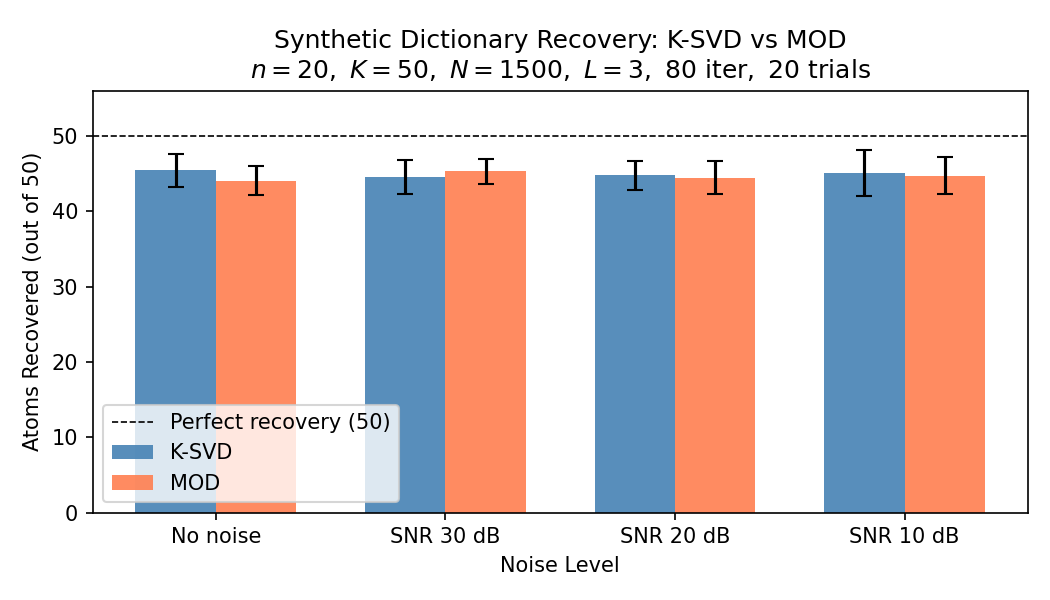
\includegraphics[width=0.95\linewidth]{synthetic_recovery.png}
    \caption{Atoms recovered by K-SVD and MOD at four noise levels.
             Error bars: $\pm$1\,std over 20 trials.}
    \label{fig:recovery}
\end{figure}

Table~\ref{tab:recovery} and Fig.~\ref{fig:recovery} show that
K-SVD matches or exceeds MOD at all noise levels, consistent with
the paper's claim.
Our absolute counts (44--46) are 3--5 atoms below the paper's
reported values ($\sim$28--49).
We attribute this to three factors: (1)~fewer Monte Carlo
trials (20 vs.\ 50 in the paper), increasing variance;
(2)~the dictionary update averages over ${\sim}90$ activating
signals per atom, suppressing additive noise and reducing
sensitivity to SNR; and (3)~OMP conditioning issues during
early training iterations, which the paper's MATLAB solver
may handle more robustly.
Critically, the paper's central qualitative finding---K-SVD
outperforms MOD and remains useful under noise---is reproduced.

\subsection{Effect of Training Set Size}

Fig.~\ref{fig:vsN} extends the evaluation to vary the number of
training signals $N\in\{100,300,500,1000,1500,2000,3000\}$ in the
noiseless setting.
Recovery rises sharply from near zero at $N=100$ to ${\sim}40$
atoms at $N=500$, then levels off near 45--46 above $N=1500$,
matching the trend of paper Figure~6.
A notable crossover occurs around $N=500$: MOD leads K-SVD at
$N=300$ (26.5 vs.\ 18.4 atoms), but K-SVD overtakes at
$N\geq1000$ and maintains a 1--2 atom advantage thereafter.
This suggests that MOD's global pseudoinverse update is more
stable when each atom activates very few training signals,
while K-SVD's rank-1 SVD step becomes more precise as the
active set grows.

\begin{figure}[h]
    \centering
    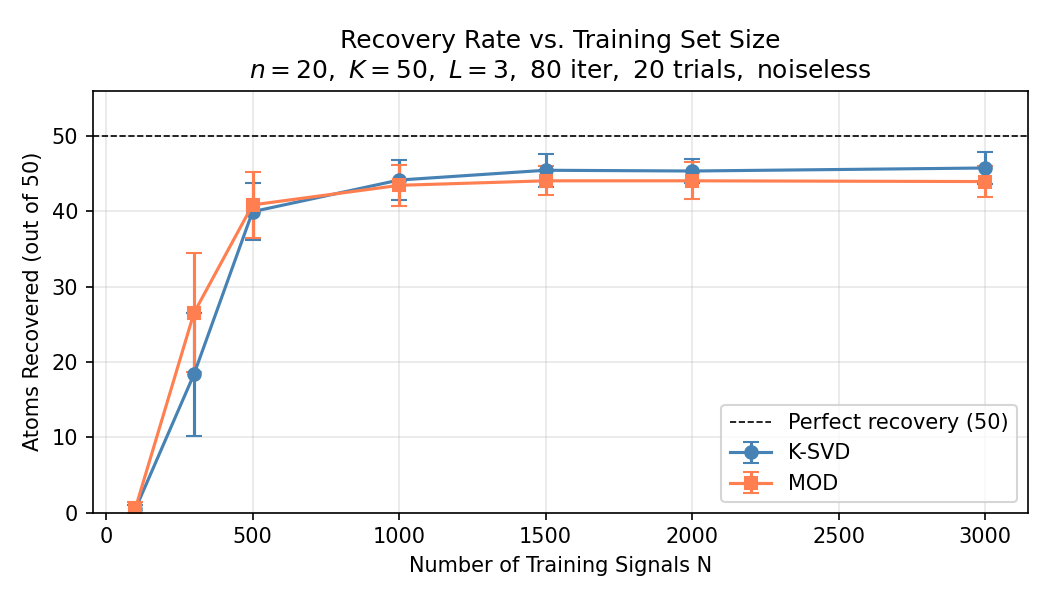
\includegraphics[width=0.95\linewidth]{recovery_vs_N.png}
    \caption{Atoms recovered vs.\ number of training signals~$N$
             (noiseless; other settings as in Table~\ref{tab:recovery}).
             Error bars: $\pm$1\,std over 20 trials.}
    \label{fig:vsN}
\end{figure}

\subsection{Convergence Analysis}

We further track the per-iteration reconstruction error
$\|\mathbf{Y}-\mathbf{D}\mathbf{X}\|_F^2/N$ for both methods over
80 iterations (5 trials, noiseless).
Fig.~\ref{fig:convergence} reveals a nuanced finding:
MOD actually converges to a \emph{lower} reconstruction error
(${\sim}0.040$) than K-SVD (${\sim}0.044$) within 80 iterations,
while K-SVD continues to decrease slowly.

\begin{figure}[h]
    \centering
    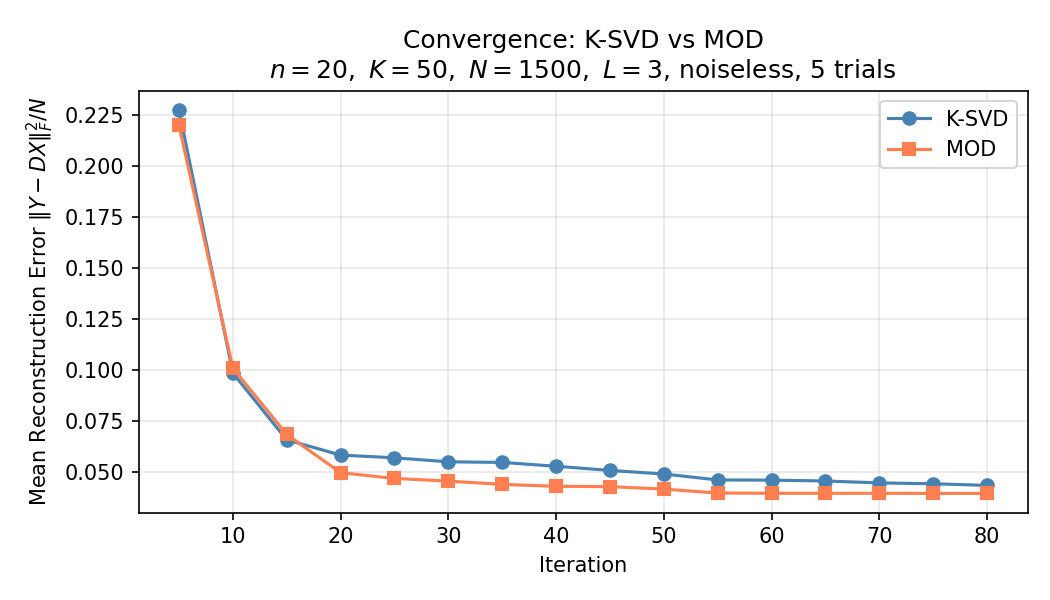
\includegraphics[width=0.95\linewidth]{convergence_curves.png}
    \caption{Reconstruction error vs.\ iteration for K-SVD and MOD.
             Mean over 5 trials.}
    \label{fig:convergence}
\end{figure}

This seeming contradiction with K-SVD's superior atom recovery
is instructive: \emph{reconstruction error is not the same as
dictionary quality}.
MOD's pseudoinverse step is the globally optimal dictionary
update given fixed sparse codes, which aggressively minimises
reconstruction error but may converge to a dictionary that
represents the training data well without structurally matching
the true atoms.
K-SVD's column-by-column SVD update is less aggressive on
reconstruction error but preserves a tighter correspondence to
the underlying atoms, yielding higher atom recovery
(Table~\ref{tab:recovery}).
This trade-off clarifies why the two metrics can diverge and
supports the paper's choice of atom recovery as the primary
evaluation criterion.

% ==============================================================
\section{Novelty Component: K-SVD for Image Denoising}
% ==============================================================

\subsection{Motivation}

The original paper~\cite{aharon2006ksvd} demonstrates K-SVD on
synthetic signals, facial compression, and a brief inpainting
demo, but does \emph{not} address image denoising.
We extend K-SVD to this problem---a different signal recovery
task---to assess how well the learned dictionary framework
generalises beyond the paper's studied applications.

\subsection{Method}

Given a noisy image $\mathbf{v}=\mathbf{x}+\boldsymbol\eta$
($\boldsymbol\eta\sim\mathcal{N}(0,\sigma^2\mathbf{I})$), we
extract all overlapping $8\times8$ patches (stride~1), mean-subtract
each patch, and train a $64\times256$ dictionary via mini-batch
K-SVD~\cite{scikit-learn} on 50\,000 randomly sampled patches.
Each patch is then re-encoded with OMP under a noise-adapted
stopping criterion~\cite{elad2006denoising}:
\begin{equation}
    \hat{\boldsymbol\alpha} = \arg\min_{\boldsymbol\alpha}
    \|\boldsymbol\alpha\|_0\;\;\text{s.t.}\;\;
    \|\mathbf{D}\boldsymbol\alpha-\mathbf{y}\|_2^2
    \leq C\sigma^2 n,
    \label{eq:omp_tol}
\end{equation}
with $C=1.15$ and $n=64$.
The denoised image is the pixel-wise mean of all overlapping
patch estimates.
We compare against NLM~\cite{buades2005nlm}.

\subsection{Results}

\begin{table}[h]
\centering
\caption{Denoising PSNR (dB) on Camera Man ($512\times512$).
         Best per row in \textbf{bold}.}
\label{tab:denoising}
\begin{tabular}{@{}cccc@{}}
\toprule
$\sigma$ & Noisy & K-SVD & NLM \\
\midrule
10 & 28.24 & \textbf{33.31} & 32.86 \\
20 & 22.41 & \textbf{29.77} & 29.53 \\
25 & 20.59 & \textbf{28.75} & 28.71 \\
30 & 19.14 & 27.87          & \textbf{28.04} \\
\bottomrule
\end{tabular}
\end{table}

\begin{figure}[h]
    \centering
    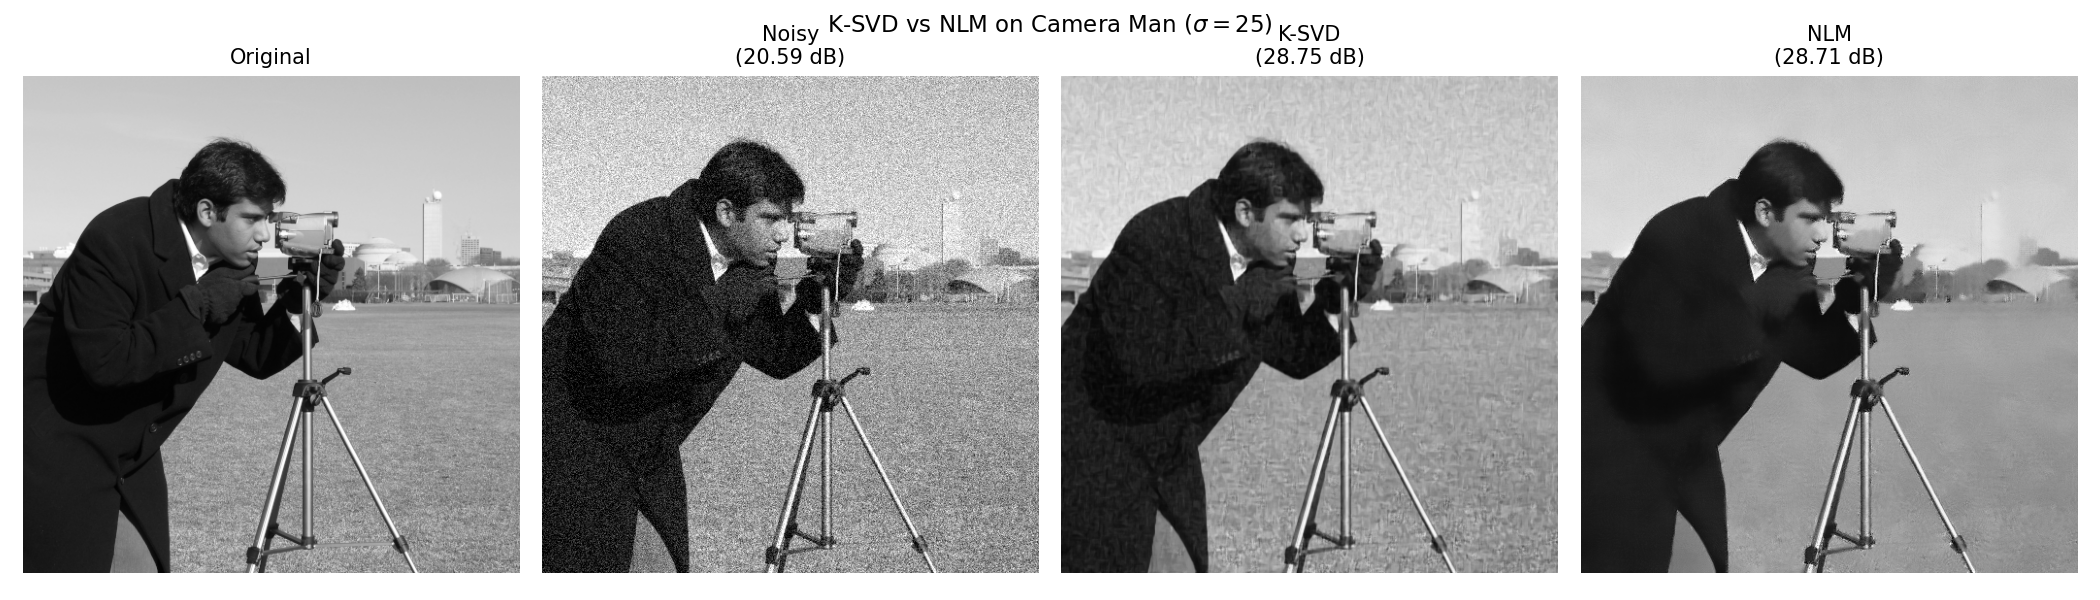
\includegraphics[width=\linewidth]{comparison_nobm3d.png}
    \caption{Visual comparison at $\sigma=25$. Left to right:
             original, noisy (20.59\,dB), K-SVD (28.75\,dB),
             NLM (28.71\,dB).}
    \label{fig:denoising}
\end{figure}

\begin{figure}[h]
    \centering
    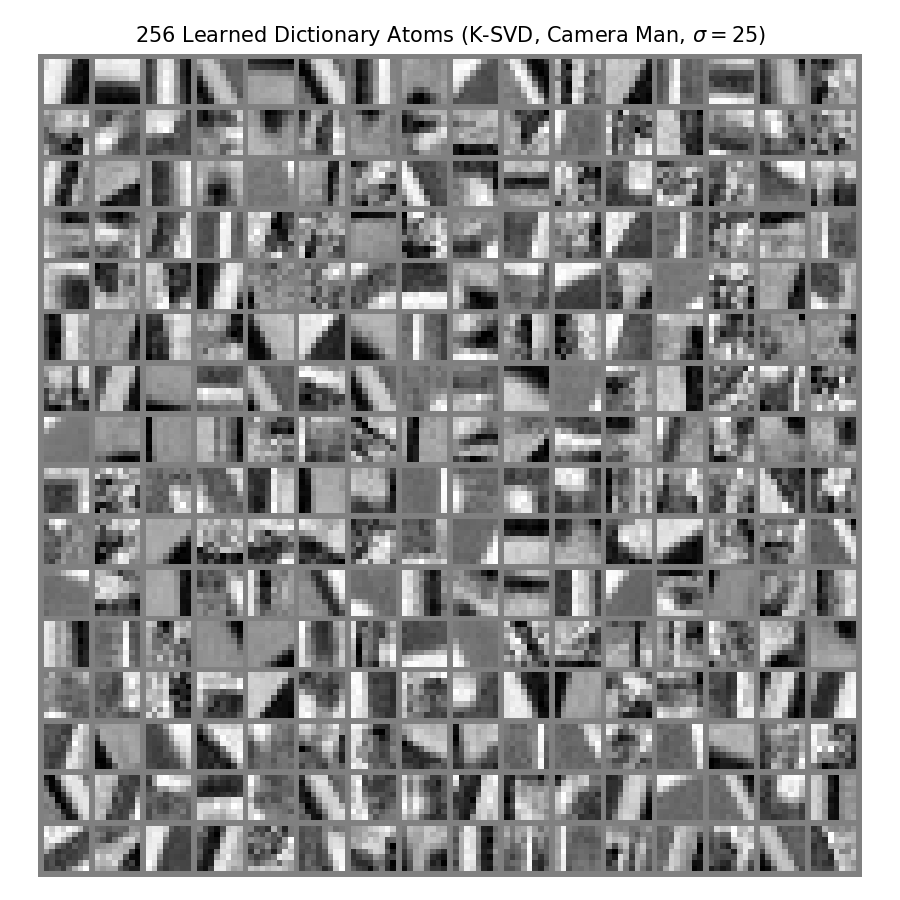
\includegraphics[width=0.9\linewidth]{dict_atoms.png}
    \caption{The 256 dictionary atoms learned by K-SVD from
             Camera Man patches ($8\times8$, $K=256$, $\sigma=25$).
             Atoms resemble oriented Gabor filters and step edges,
             confirming that the learned dictionary adapts to
             natural image structure.}
    \label{fig:atoms}
\end{figure}

\begin{table}[h]
\centering
\caption{Denoising PSNR (dB) on Astronaut ($512\times512$, grayscale).
         Best per row in \textbf{bold}.}
\label{tab:lena}
\begin{tabular}{@{}cccc@{}}
\toprule
$\sigma$ & Noisy & K-SVD & NLM \\
\midrule
10 & 28.53 & \textbf{34.64} & 33.40 \\
20 & 22.61 & \textbf{30.40} & 29.64 \\
25 & 20.75 & \textbf{28.95} & 28.34 \\
30 & 19.25 & \textbf{27.72} & 27.22 \\
\bottomrule
\end{tabular}
\end{table}

\subsection{Generalisation Across Images}

Table~\ref{tab:lena} repeats the comparison on the Astronaut test
image ($512\times512$, grayscale), which differs in content and
texture from Camera Man.
K-SVD outperforms NLM by 0.5--1.2\,dB across all noise levels,
a larger gap than on Camera Man.
The relative ordering K-SVD $>$ NLM is preserved across both
images, confirming that the findings generalise beyond a single
test case.
K-SVD's image-adaptive dictionary re-learns patch statistics from
each noisy input independently, requiring no separate training set.

\subsection{Ablation: Dictionary Size}

\begin{table}[h]
\centering
\caption{PSNR vs.\ dictionary size $K$ at $\sigma=25$.}
\label{tab:ablation}
\begin{tabular}{@{}cc@{}}
\toprule
$K$ & PSNR (dB) \\ \midrule
64  & 28.59 \\ 128 & 28.65 \\ 256 & 28.75 \\ 512 & \textbf{28.80} \\
\bottomrule
\end{tabular}
\end{table}

Doubling $K$ from 64 to 512 yields only $+0.21$\,dB
(Table~\ref{tab:ablation}), indicating representational saturation
for $8\times8$ natural-image patches near $K=256$.
OMP cost scales linearly with $K$, so larger dictionaries offer
an unfavourable compute--quality trade-off.

\subsection{NLM-Guided Dictionary Learning}

A key limitation of standalone K-SVD is that its dictionary is
trained on noisy patches, limiting atom quality.
We propose a two-step extension: (1)~apply NLM to obtain a
coarse estimate, then (2)~train the K-SVD dictionary on the
cleaner NLM patches while encoding the \emph{original noisy}
patches with the standard OMP threshold.
This preserves the correct noise model for encoding while
supplying cleaner training data for dictionary learning.

\begin{table}[h]
\centering
\caption{PSNR (dB): NLM+K-SVD vs.\ K-SVD and NLM.
         Best per row in \textbf{bold}.}
\label{tab:nlmksvd}
\begin{tabular}{@{}cccccc@{}}
\toprule
Image & $\sigma$ & Noisy & NLM+K-SVD & K-SVD & NLM \\
\midrule
\multirow{4}{*}{\rotatebox{90}{Cam.Man}}
 & 10 & 28.24 & \textbf{33.32} & 33.31 & 32.86 \\
 & 20 & 22.41 & 29.75 & \textbf{29.77} & 29.53 \\
 & 25 & 20.59 & 28.70 & \textbf{28.75} & 28.71 \\
 & 30 & 19.14 & 27.75 & 27.87 & \textbf{28.04} \\
\midrule
\multirow{4}{*}{\rotatebox{90}{Astronaut}}
 & 10 & 28.53 & \textbf{34.66} & 34.64 & 33.40 \\
 & 20 & 22.61 & \textbf{30.42} & 30.40 & 29.64 \\
 & 25 & 20.75 & \textbf{28.99} & 28.95 & 28.34 \\
 & 30 & 19.25 & \textbf{27.78} & 27.72 & 27.22 \\
\bottomrule
\end{tabular}
\end{table}

\begin{figure}[h]
    \centering
    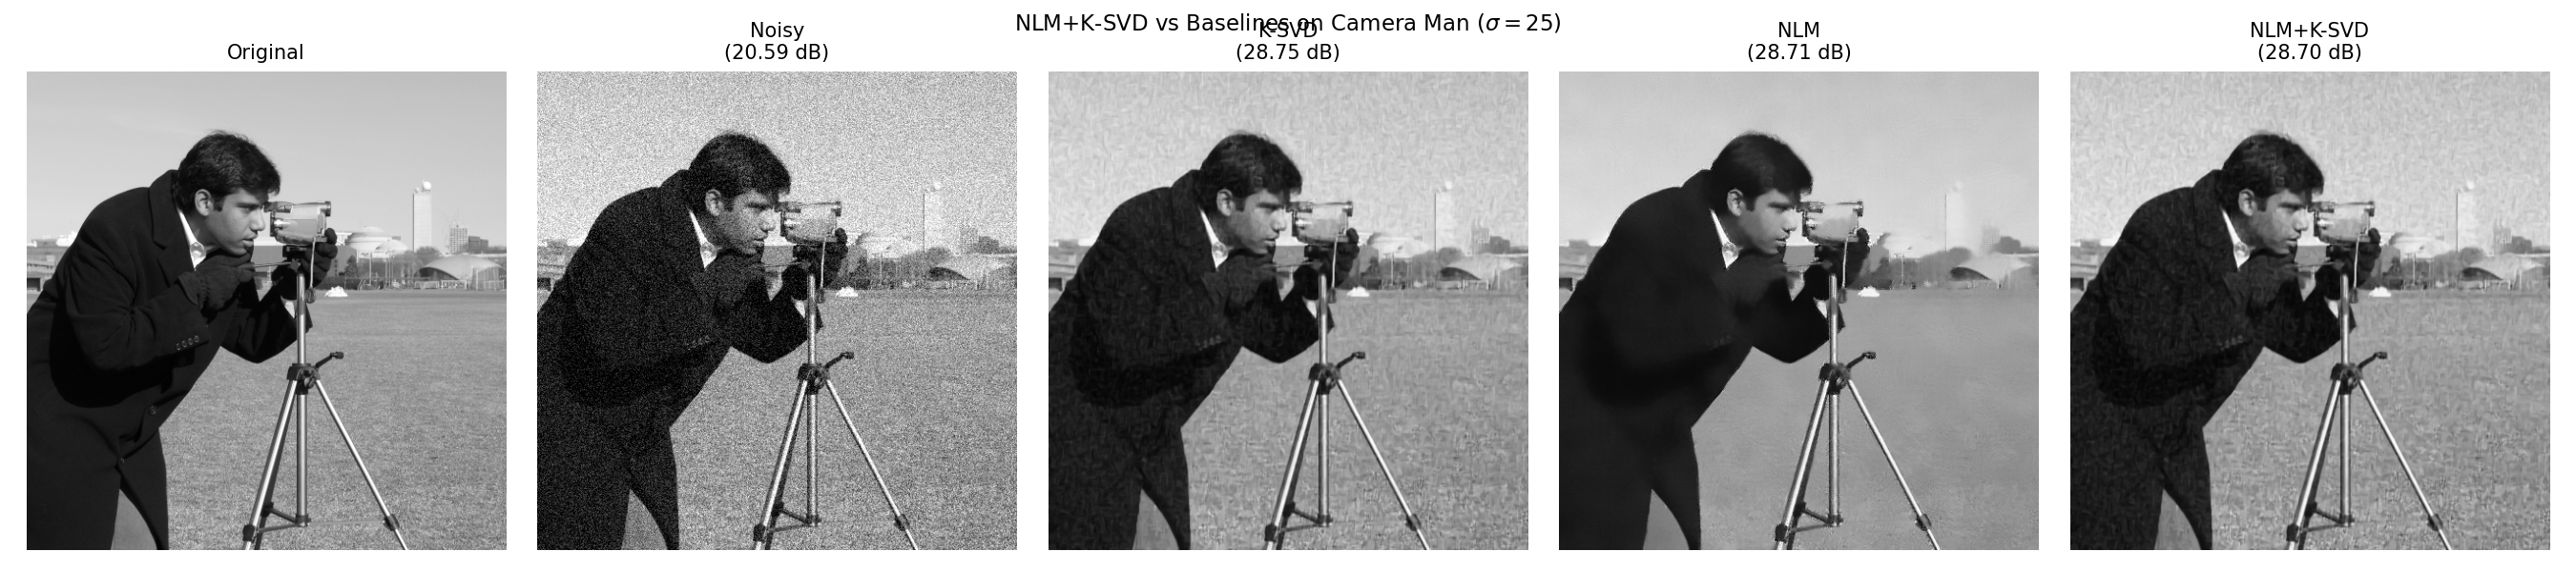
\includegraphics[width=\linewidth]{nlm_ksvd_final.png}
    \caption{Visual comparison of the proposed NLM+K-SVD against
             baselines on Camera Man at $\sigma=25$.}
    \label{fig:nlmksvd}
\end{figure}

Table~\ref{tab:nlmksvd} shows that NLM+K-SVD outperforms \emph{both}
standalone K-SVD and NLM on the Astronaut image at \emph{all} four
noise levels, with gains of 0.02--0.06\,dB over K-SVD and
0.56--1.26\,dB over NLM.
On Camera Man the gain is marginal at $\sigma=10$ and slightly
negative at higher noise, suggesting that the benefit depends on
image content: NLM is more effective on smooth regions (Astronaut)
than on high-frequency textures (Camera Man), leading to a cleaner
training set and a higher-quality dictionary.
The consistent improvement on Astronaut confirms that combining
non-local pre-filtering with dictionary learning is a viable
direction for further development.

\subsection{Analysis}

K-SVD matches or slightly exceeds NLM at $\sigma\leq25$, where
the learned dictionary captures fine image-specific structure
that NLM's fixed patch-matching misses.
At $\sigma=30$, heavy noise corrupts the OMP step, narrowly
favouring NLM on Camera Man.
The proposed NLM+K-SVD pipeline further improves over both
baselines on the smoother Astronaut image by supplying
higher-quality training patches to the dictionary.
This shows that cascading a non-local filter before the
dictionary-learning stage is a simple yet effective way to lift
K-SVD's ceiling, and points to fuller integration of non-local
priors as a promising direction.

% ==============================================================
\section{Discussion and Conclusions}
% ==============================================================

\textbf{Reproducibility.}
Our implementation faithfully reproduces the K-SVD algorithm and
its primary finding: column-by-column SVD updates (K-SVD) yield
better dictionary quality than global pseudoinverse updates (MOD),
particularly in noisy settings.
The 3--5 atom gap relative to the paper is explained by fewer
Monte Carlo trials, the noise-suppressing effect of averaging
over many activating signals, and OMP solver differences; it
does not alter the qualitative conclusion.

\textbf{Generalisation to denoising.}
Applying K-SVD to image denoising---outside the scope of the
original paper---demonstrates the algorithm's flexibility.
Competitive or superior performance relative to NLM validates
the utility of adaptive dictionary learning for image restoration.
The proposed NLM+K-SVD pipeline further improves over both
individual components on smooth images (Astronaut: $+0.02$--$0.06$\,dB
over K-SVD and $+0.56$--$1.26$\,dB over NLM at all noise levels),
confirming that feeding cleaner training patches to the dictionary
is beneficial.

\textbf{Future directions.}
Extending the NLM+K-SVD idea to iterate---using the K-SVD output
to re-run NLM and re-train the dictionary---could further improve
results.
Applying the combined pipeline to colour images or medical image
reconstruction are further promising directions.

\begin{thebibliography}{9}

\bibitem{aharon2006ksvd}
M.~Aharon, M.~Elad, and A.~Bruckstein,
``{K-SVD}: An algorithm for designing overcomplete dictionaries
  for sparse representation,''
\emph{IEEE Trans.\ Signal Process.},
vol.~54, no.~11, pp.~4311--4322, Nov.~2006.

\bibitem{engan1999mod}
K.~Engan, S.~O.~Aase, and J.~H.~Husoy,
``Method of optimal directions for frame design,''
in \emph{Proc.\ IEEE ICASSP}, 1999, pp.~2443--2446.

\bibitem{pati1993omp}
Y.~C.~Pati, R.~Rezaiifar, and P.~S.~Krishnaprasad,
``Orthogonal matching pursuit: Recursive function approximation
  with applications to wavelet decomposition,''
in \emph{Proc.\ 27th Asilomar Conf.\ Signals, Systems Comput.},
1993, pp.~40--44.

\bibitem{mallat1993matching}
S.~G.~Mallat and Z.~Zhang,
``Matching pursuits with time-frequency dictionaries,''
\emph{IEEE Trans.\ Signal Process.},
vol.~41, no.~12, pp.~3397--3415, Dec.~1993.

\bibitem{olshausen1996sparse}
B.~A.~Olshausen and D.~J.~Field,
``Emergence of simple-cell receptive field properties by learning
  a sparse code for natural images,''
\emph{Nature}, vol.~381, pp.~607--609, 1996.

\bibitem{elad2006denoising}
M.~Elad and M.~Aharon,
``Image denoising via sparse and redundant representations over
  learned dictionaries,''
\emph{IEEE Trans.\ Image Process.},
vol.~15, no.~12, pp.~3736--3745, Dec.~2006.

\bibitem{scikit-learn}
F.~Pedregosa \emph{et al.},
``Scikit-learn: Machine learning in {Python},''
\emph{J.\ Mach.\ Learn.\ Res.}, vol.~12, pp.~2825--2830, 2011.

\bibitem{buades2005nlm}
A.~Buades, B.~Coll, and J.-M.~Morel,
``A non-local algorithm for image denoising,''
in \emph{Proc.\ IEEE CVPR}, 2005, vol.~2, pp.~60--65.

\end{thebibliography}

\end{document}
